%
%	Praxisbezug
%

\pagebreak
\section{CIS Scans}

\onehalfspacing

\subsection{Rancher hardening}

Text.\footnote{See \textit{Rancher Labs (2019)}: Hardening Guide. \cite{hardeningGuide}}

\subsection{CIS Scan GUI}

Text. 

\begin{figure}[H]
\centering
\caption {CIS Scan GUI}
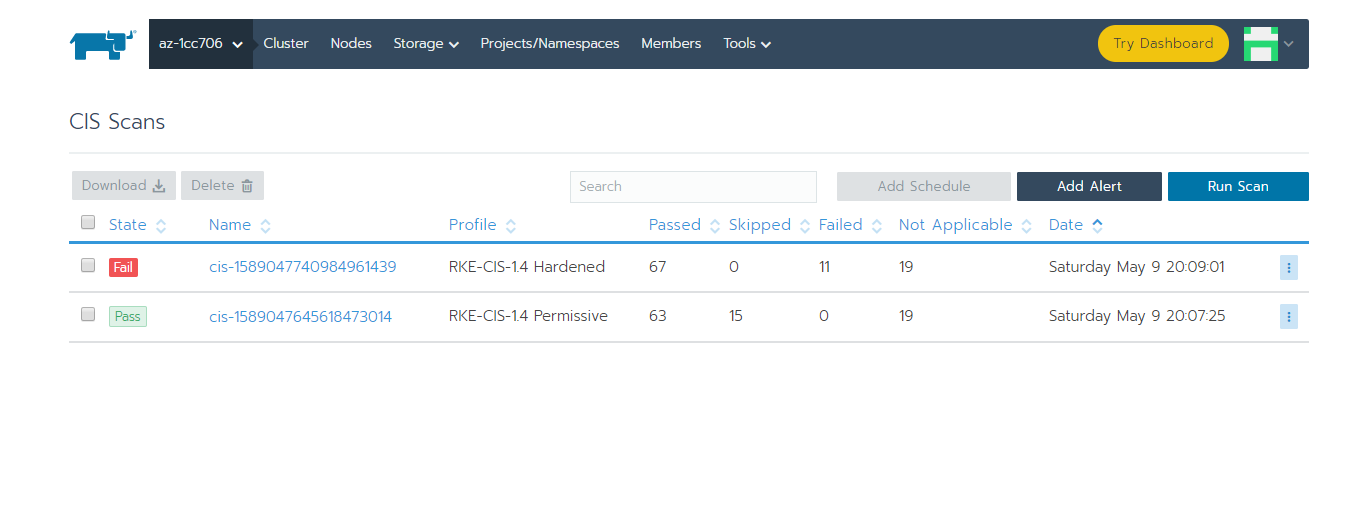
\includegraphics[width=\linewidth]{images/cis-scan-overview.png}
\label{fig:cisScanOverview}
\end{figure}

\subsection{CIS Scan Hardened}

Text. 

\begin{figure}[H]
\centering
\caption {CIS Scan Hardened}
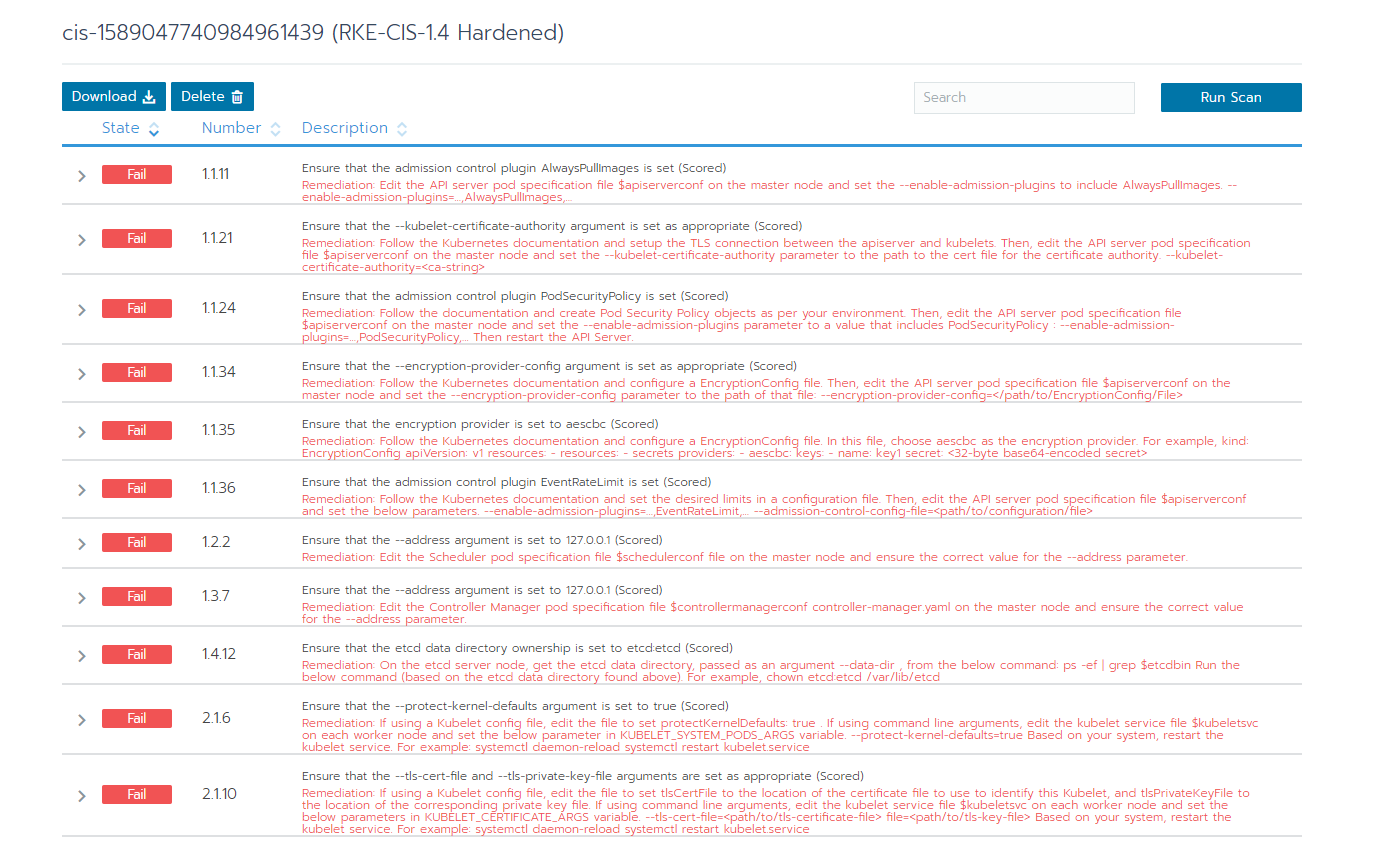
\includegraphics[width=\linewidth]{images/cis-scan-detail.png}
\label{fig:cisScanDetails}
\end{figure}

\subsection{Remediation}

Text.\footnote{See \textit{Rancher Labs (2020)}: Changelog. \cite{ChangeLog}}

Text.\footnote{See \textit{Price, J. (2020)}: Kubernetes - Pod Security Policies. \cite{examplePsp}}

Text.\footnote{See \textit{Iradier, A. (2020)}: Enhancing Kubernetes Security with Pod Security Policies. \cite{detailPsp}}

Text.\footnote{See \textit{Shankar, P. (2020)}: Runtime Security in Rancher with Falco. \cite{falcoPsp}}
